
\section{Setup Eclipse}

Setting up a Maven multiple-project hierarchy is not difficult. All it
takes are 6 easy steps:

\begin{enumerate}
\def\labelenumi{\arabic{enumi}.}
\item
  Download and install the
  \href{https://www.eclipse.org/downloads/}{Eclipse}-IDE (integrated
  development environment), if you don't have already. You can use the
  standard edition.
\item
  Download and unzip the newest
  \href{https://github.com/a-d/spatial.election/archive/master.zip}{spatial.election}
  files.
\item
  Start Eclipse. 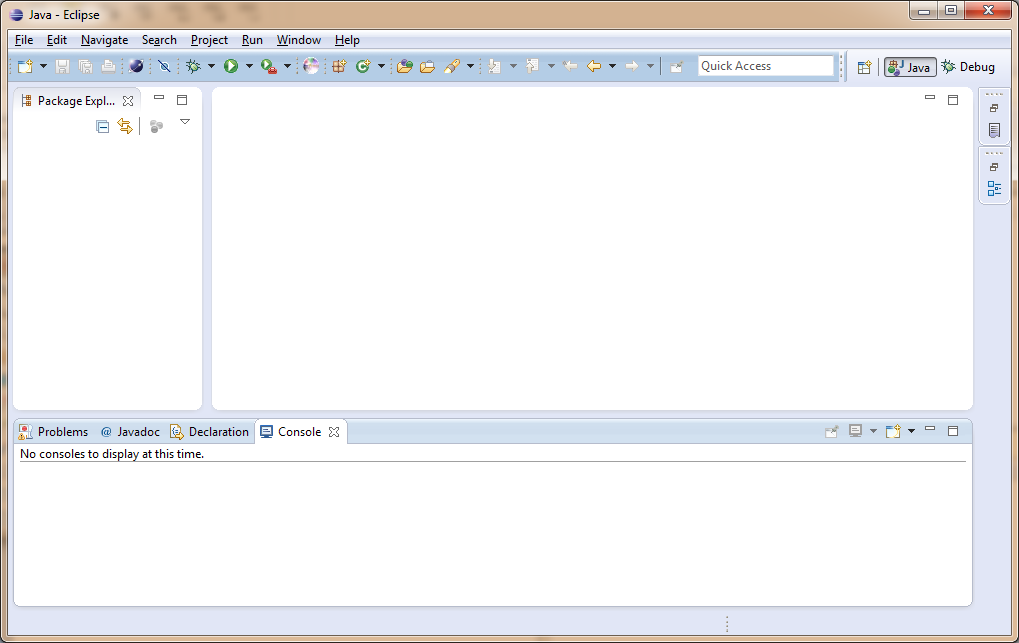
\includegraphics[width=1.1\textwidth]{../img/GMXSI1f.png}
\item
  Check whether M2E is installed. It's a plugin for eclipse, providing
  Maven features. Go to \textbf{Help} -\textgreater{} \textbf{Install
  New Software}. Enter the site ``\textbf{M2E -
  !http://download.eclipse.org/technology/m2e/releases}''. Install
  ``Maven Integration for Eclipse'' if it is not yet installed. Restart
  Eclipse if necessary.

  \begin{figure}[htbp]
  \centering
  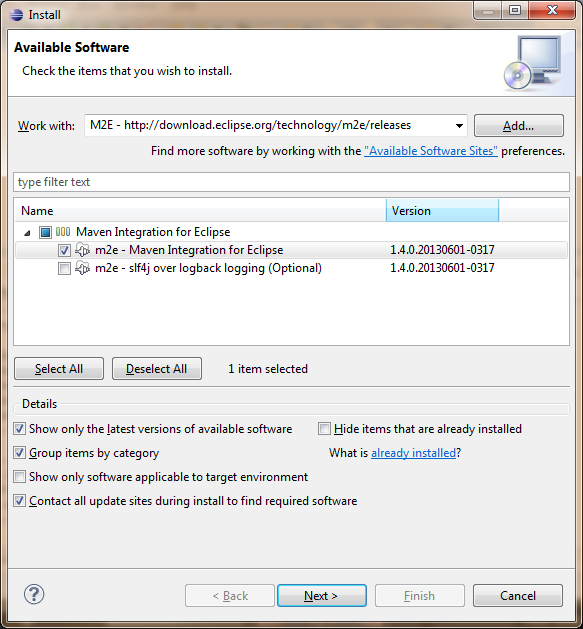
\includegraphics[width=1.1\textwidth]{../img/nO8HPxH.png}
  \caption{eclipse m2e}
  \end{figure}
\item
  Import the \emph{spatial.election} project, by using \textbf{File}
  -\textgreater{} \textbf{Import}, check ``Existing Maven Projects''.
  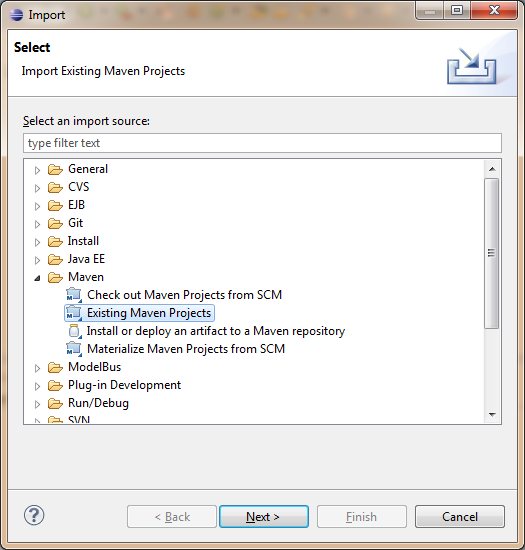
\includegraphics[width=1.1\textwidth]{../img/OozCHLd.png}
\item
  Enter the path to your unziped \emph{spatial.election} files. Check
  all projects and skip through the following \emph{Import} dialogs.
  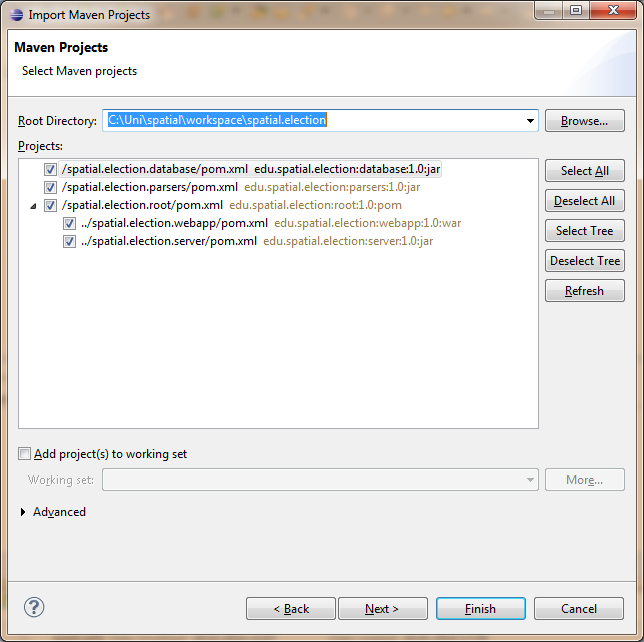
\includegraphics[width=1.1\textwidth]{../img/vBZ4xNA.png}
\end{enumerate}

\begin{center}\rule{3in}{0.4pt}\end{center}

Congratulation, you've did it! Now you are ready to use the
\emph{spatial.election} software with source code. You can alter the
code, as well as build and run the application. If you already have
{[}{[}Setup the PostgreSQL server\textbar{}Setup-PostgreSQL{]}{]} you
can go on learning how to {[}{[}use the software\textbar{}Running{]}{]}.

\begin{figure}[htbp]
\centering
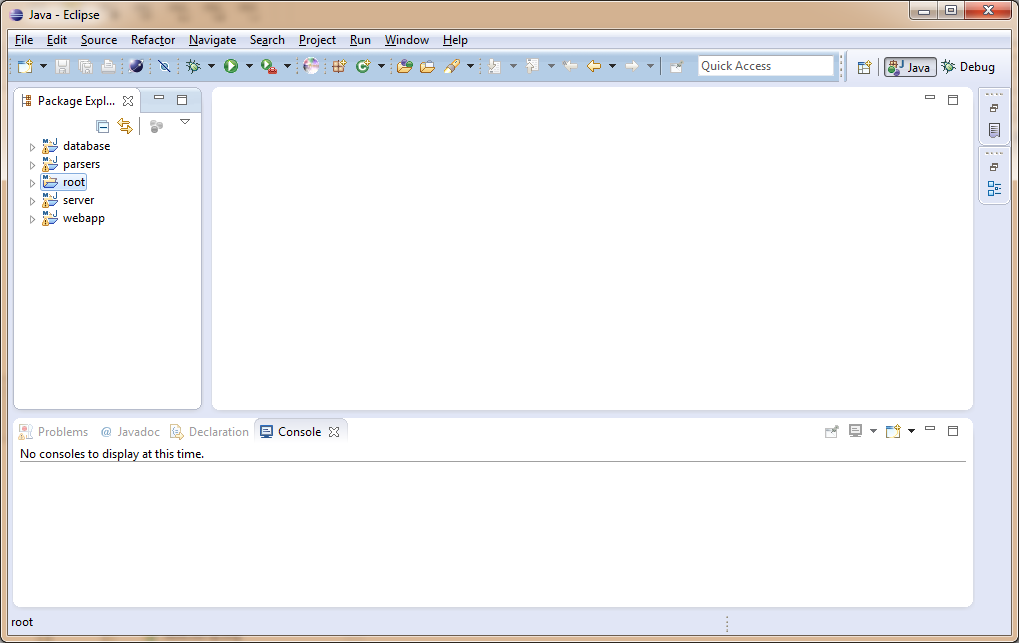
\includegraphics[width=1.1\textwidth]{../img/EeGnXjg.png}
\caption{eclipse ready}
\end{figure}